\setcounter{page}{-9}
%%% Platnica
\begin{otherlanguage}{slovene}
\begin{center}
\pagestyle{empty}
{\large UNIVERZA V LJUBLJANI\\
FAKULTETA ZA MATEMATIKO IN FIZIKO
}

\vspace{7cm}

{\huge DOKTORSKA DISERTACIJA}

\vspace{5cm}

\tikzfading[name=fade out,
inner color=transparent!0,
outer color=transparent!0]
% Now we use the fading in another picture:
\begin{tikzpicture}[remember picture, overlay]
\node[opacity=1.0,inner sep=0pt, scope fading=fade out] at (0,-2)
{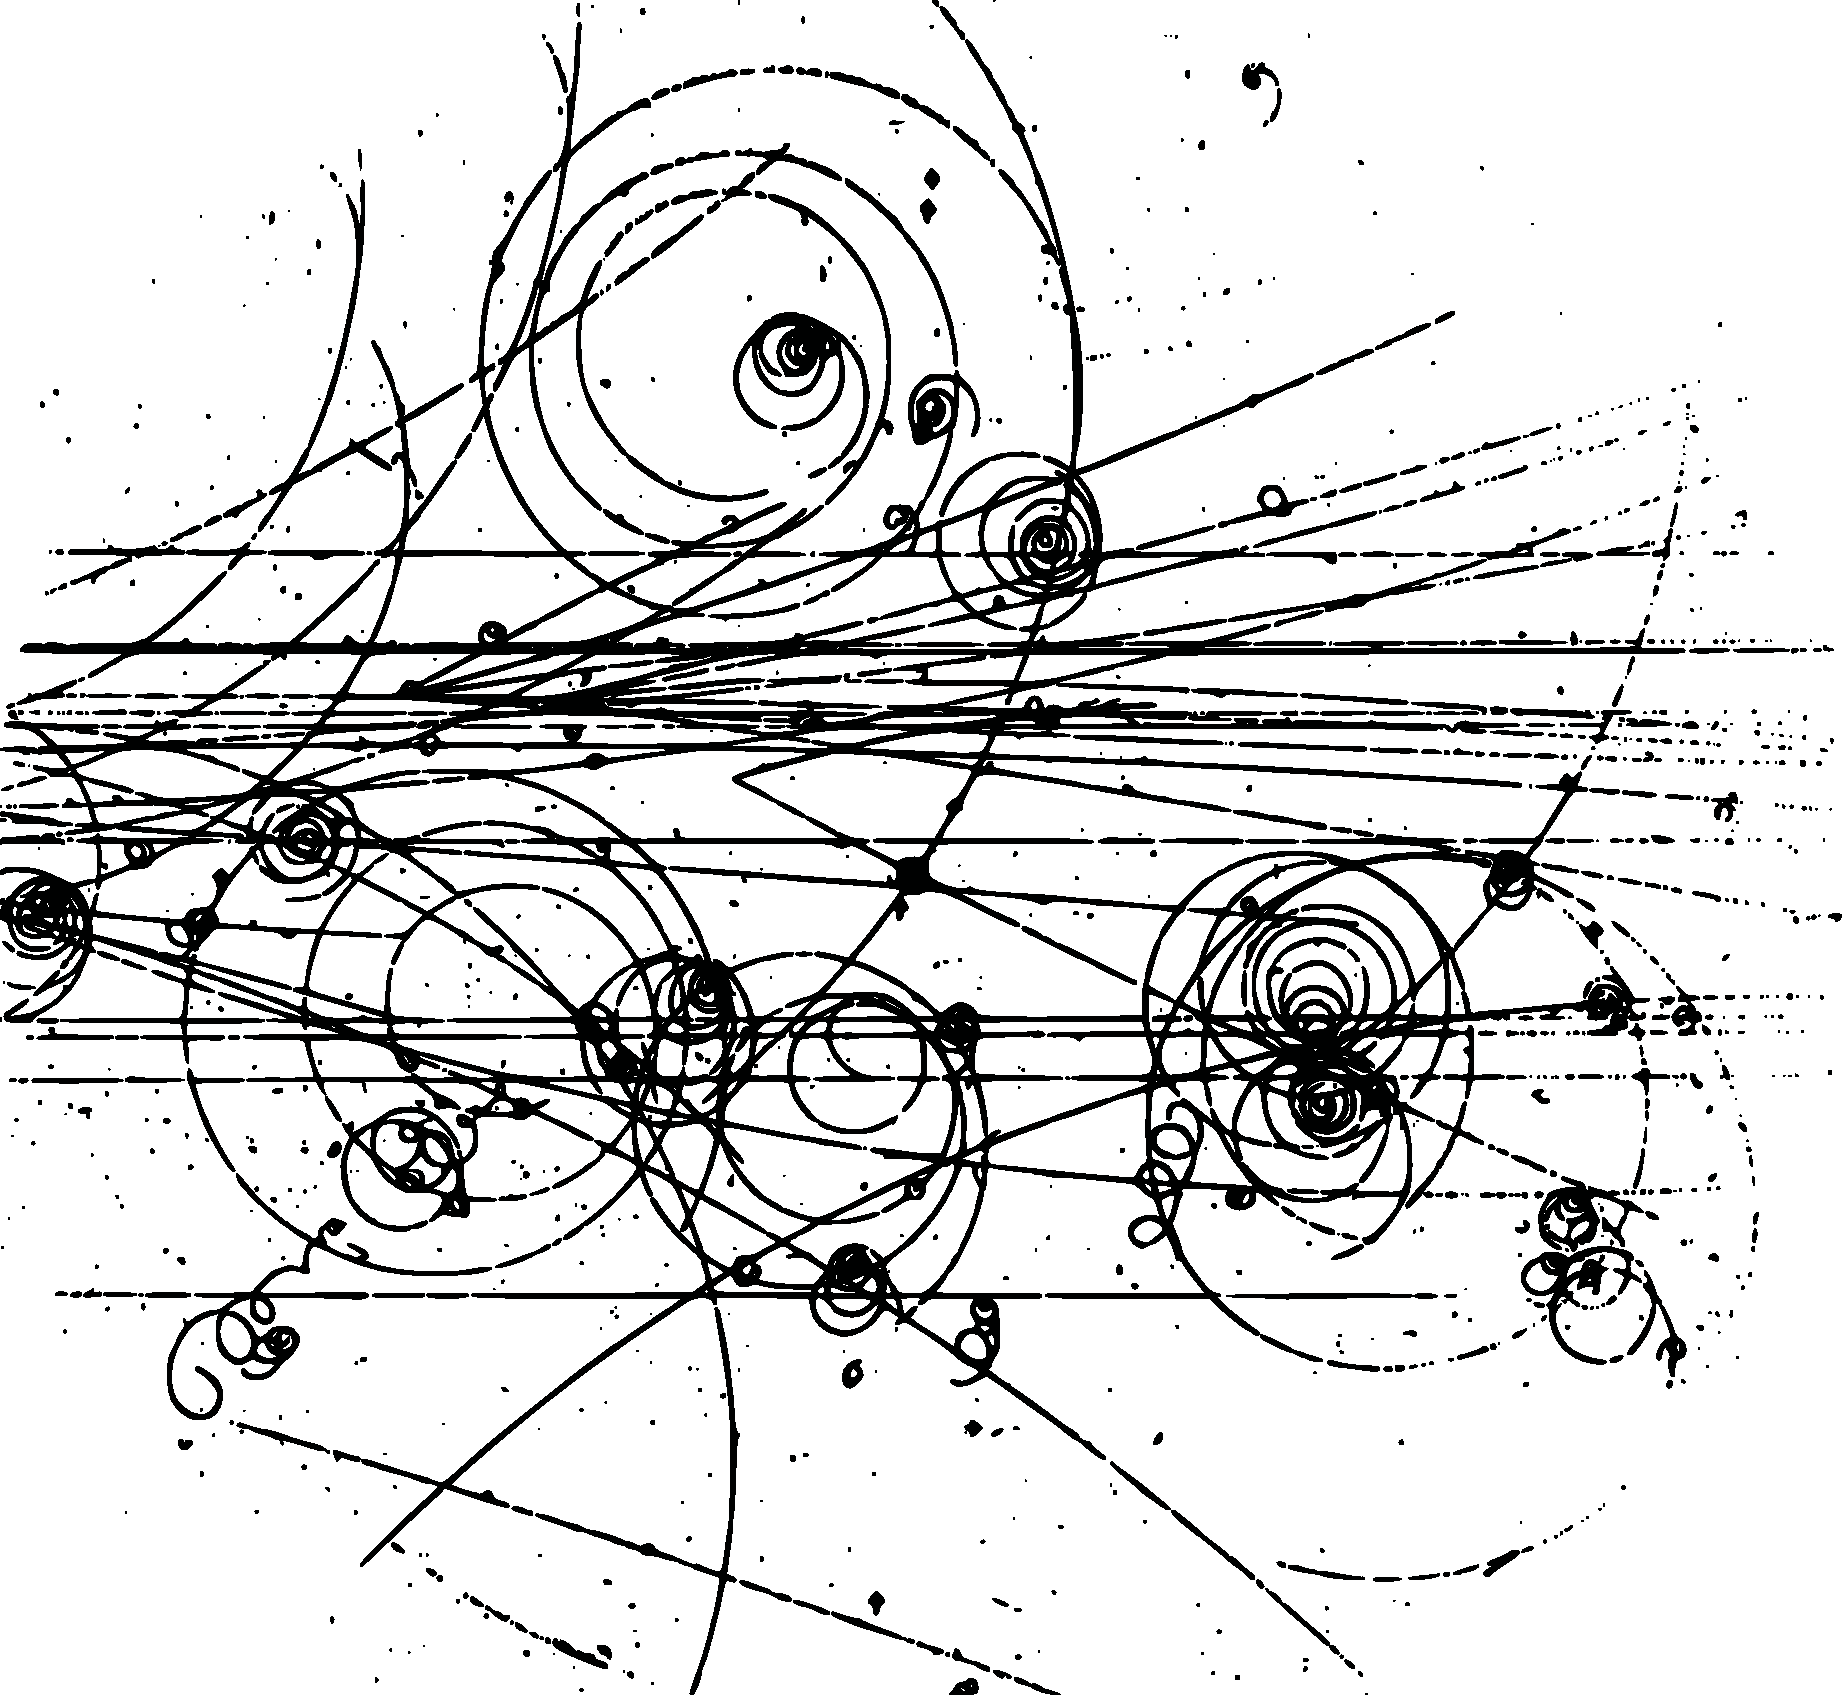
\includegraphics[width=0.6\linewidth]{fig/bc_1}};
\end{tikzpicture}

\vfill

{\hfill \large Matic Lubej}

\vspace{1cm}
{\large 2018}

\cleardoublepage

\end{center}
\end{otherlanguage}

%%% NASLOVNA STRAN V ANGLESKEM JEZIKU
\pagenumbering{roman}
\pagestyle{empty}
\begin{center}


\includegraphics[trim={0 0 0 2cm},clip]{fig/logo}

{\large UNIVERSITY OF LJUBLJANA\\
FACULTY OF MATHEMATICS AND PHYSICS\\
DEPARTMENT OF PHYSICS\\}

\vspace{5cm}

{\Large Matic Lubej\\}

\vspace{10mm}

{\bf \Large Measurement of the $\bm{B^+ \to K^+K^-\ell^+\nu_\ell}$ Decay with the Belle Detector\\}
\vspace{5mm}
{\large Doctoral thesis}\\

\vfill

{\large ADVISER: Assist. Prof. Dr. An\v ze Zupanc\\
%COADVISER: Ime in priimek\\
}

\vspace{2cm}
{\large Ljubljana, 2018}

\end{center}


%%% NASLOVNA STRAN V SLOVENSKEM JEZIKU

\cleardoublepage
\begin{otherlanguage}{slovene}
\begin{center}


\includegraphics[trim={0 0 0 2cm},clip]{fig/logo}

{\large UNIVERZA V LJUBLJANI\\
FAKULTETA ZA MATEMATIKO IN FIZIKO\\
ODDELEK ZA FIZIKO\\}

\vspace{5cm}

{\Large Matic Lubej\\}

\vspace{10mm}

{\bf \Large Meritev razpada $\bm{B^+ \to K^+K^-\ell^+\nu_\ell}$ z detektorjem Belle\\}
\vspace{5mm}
{\large Doktorska disertacija}\\

\vfill

{\large MENTOR: doc. dr. An\v ze Zupanc\\
%SOMENTOR$\backslash$-ICA: naziv, Ime in priimek\\
}



\vspace{2cm}

{\large Ljubljana, 2018}

\end{center}


%%% ZAHVALA (NEOBVEZNO)

\cleardoublepage

\pagestyle{plain}
\vfill
\chapter*{Zahvala}
Na tem mestu zapi"site, komu se zahvaljujete za pomo"c 
pri nastanku doktorske disertacije.
\pagestyle{empty}

%%% IZVLECEK

\cleardoublepage
\chapter*{Izvle"cek}
Kratek izvle"cek v slovenskem jeziku.\\
\vspace{1cm}\\
{\bf Klju"cne besede:}\\
{\bf PACS:}
\end{otherlanguage}

\pagestyle{empty}

%%% ABSTRACT
\cleardoublepage
\pagestyle{plain}
\chapter*{Abstract}
Kratek izvle"cek v angle"skem jeziku.
\vspace{1cm}\\
{\bf Keywords:}\\
{\bf PACS:}

\pagestyle{empty}

%%% KAZALO
\tableofcontents
\pagestyle{plain}
